\section{Erste Schritte}\label{s:ErsteSchritte}

Um den Umgang mit den SunSPOTs zu erlernen und ihre Software und Hardware kennen zu lernen, bietet Oracle auf der Website eine Anleitung inklusive Übungen an, welche sukzessive abgearbeitet werden kann. Die Anleitung umfasst die Installation der Software sowie das Ausführen von Testprogrammen, welche die Fähigkeiten des SunSPOTs demonstrieren.

\subsection{Installation}\label{s:Installation}

Zur Installation der Verwaltungsapplikation 'SunSPOT Manager' und dem Sun\-SPOT SDK, mit welchem man die Programm für die SunSPOTs schreibt, startet man das 'SunSPOT Manager Java Webstart' Programm. Das Webstart-Programm lädt darauf hin den Manager und das SDK herunter und installiert es auf der Workstation. Zur einwandfreien Benutzung des Managers müssen folgende Tools vorhanden sein:

\begin{itemize}
	\item ein aktuelles Java Development Kit
	\item Apache ANT
	\item optional: NetBeans IDE
\end{itemize}

Das Installationsprogramm weist auf ein Fehlen oben genannter Tools hin und installiert diese bei Bedarf nach. Sollte dies nicht automatisch durch das Programm geschehen, können diese Programme auch manuell nachinstalliert werden.
Während der Installation wird nach dem SunSPOT SDK gefragt, welches installiert werden soll. Je nach Version der SPOTs ist hier die entsprechende Version auszuwählen.\\

Normalerweise wird beim Anschließen per USB der entsprechende Treiber für die SPOTs automatisch installiert. Bei aktuellen 64-bit Windows-Versionen (7/8/8.1) kommt es allerdings zu Schwierigkeiten. Eine spezielle Treiber-Datei wurde am 7. Mai 2010 durch Bob Alkire im Oracle-Blog veröffentlicht und kann dort heruntergeladen werden. Mit ihr ist es möglich, die SPOTs auch mit aktuellen 64-bit Windows-Plattformen zu verwenden \cite{ws:alkire}.\\

Sobald der Manager und alle zugehörigen Treiber erfolgreich installiert wurden, können Programme mit Hilfe von NetBeans oder einer anderen IDE geschrieben und auf den SPOT übertragen werden.

\subsection{Übung - Flashlight}\label{s:Uebung1}

In der ersten Übung soll das erste Beispielprogramm 'Flashlight' auf den SPOT übertragen, dort ausgeführt und die zugehörigen Programmausgaben (Konsolen- \& Debugausgaben) betrachtet werden. 

Nach dem erfolgreichen Übertragen des Programms blinken die LEDs des SPOTs in kurzem Abstand, vorausgesetzt, es wird ein bestimmter Helligkeitswert, ausgelesen vom Lichtsensor, nicht überschritten. Mit Hilfe des rechten Knopfschalters auf dem Sensorboard kann außerdem die Farbe der LEDs geändert werden. Die Konsolenausgabe des Programms besteht aus dem momentanen Helligkeitswert, der vom Lichtsensor erfasst wird.

\begin{figure}[H] 
	\centering
	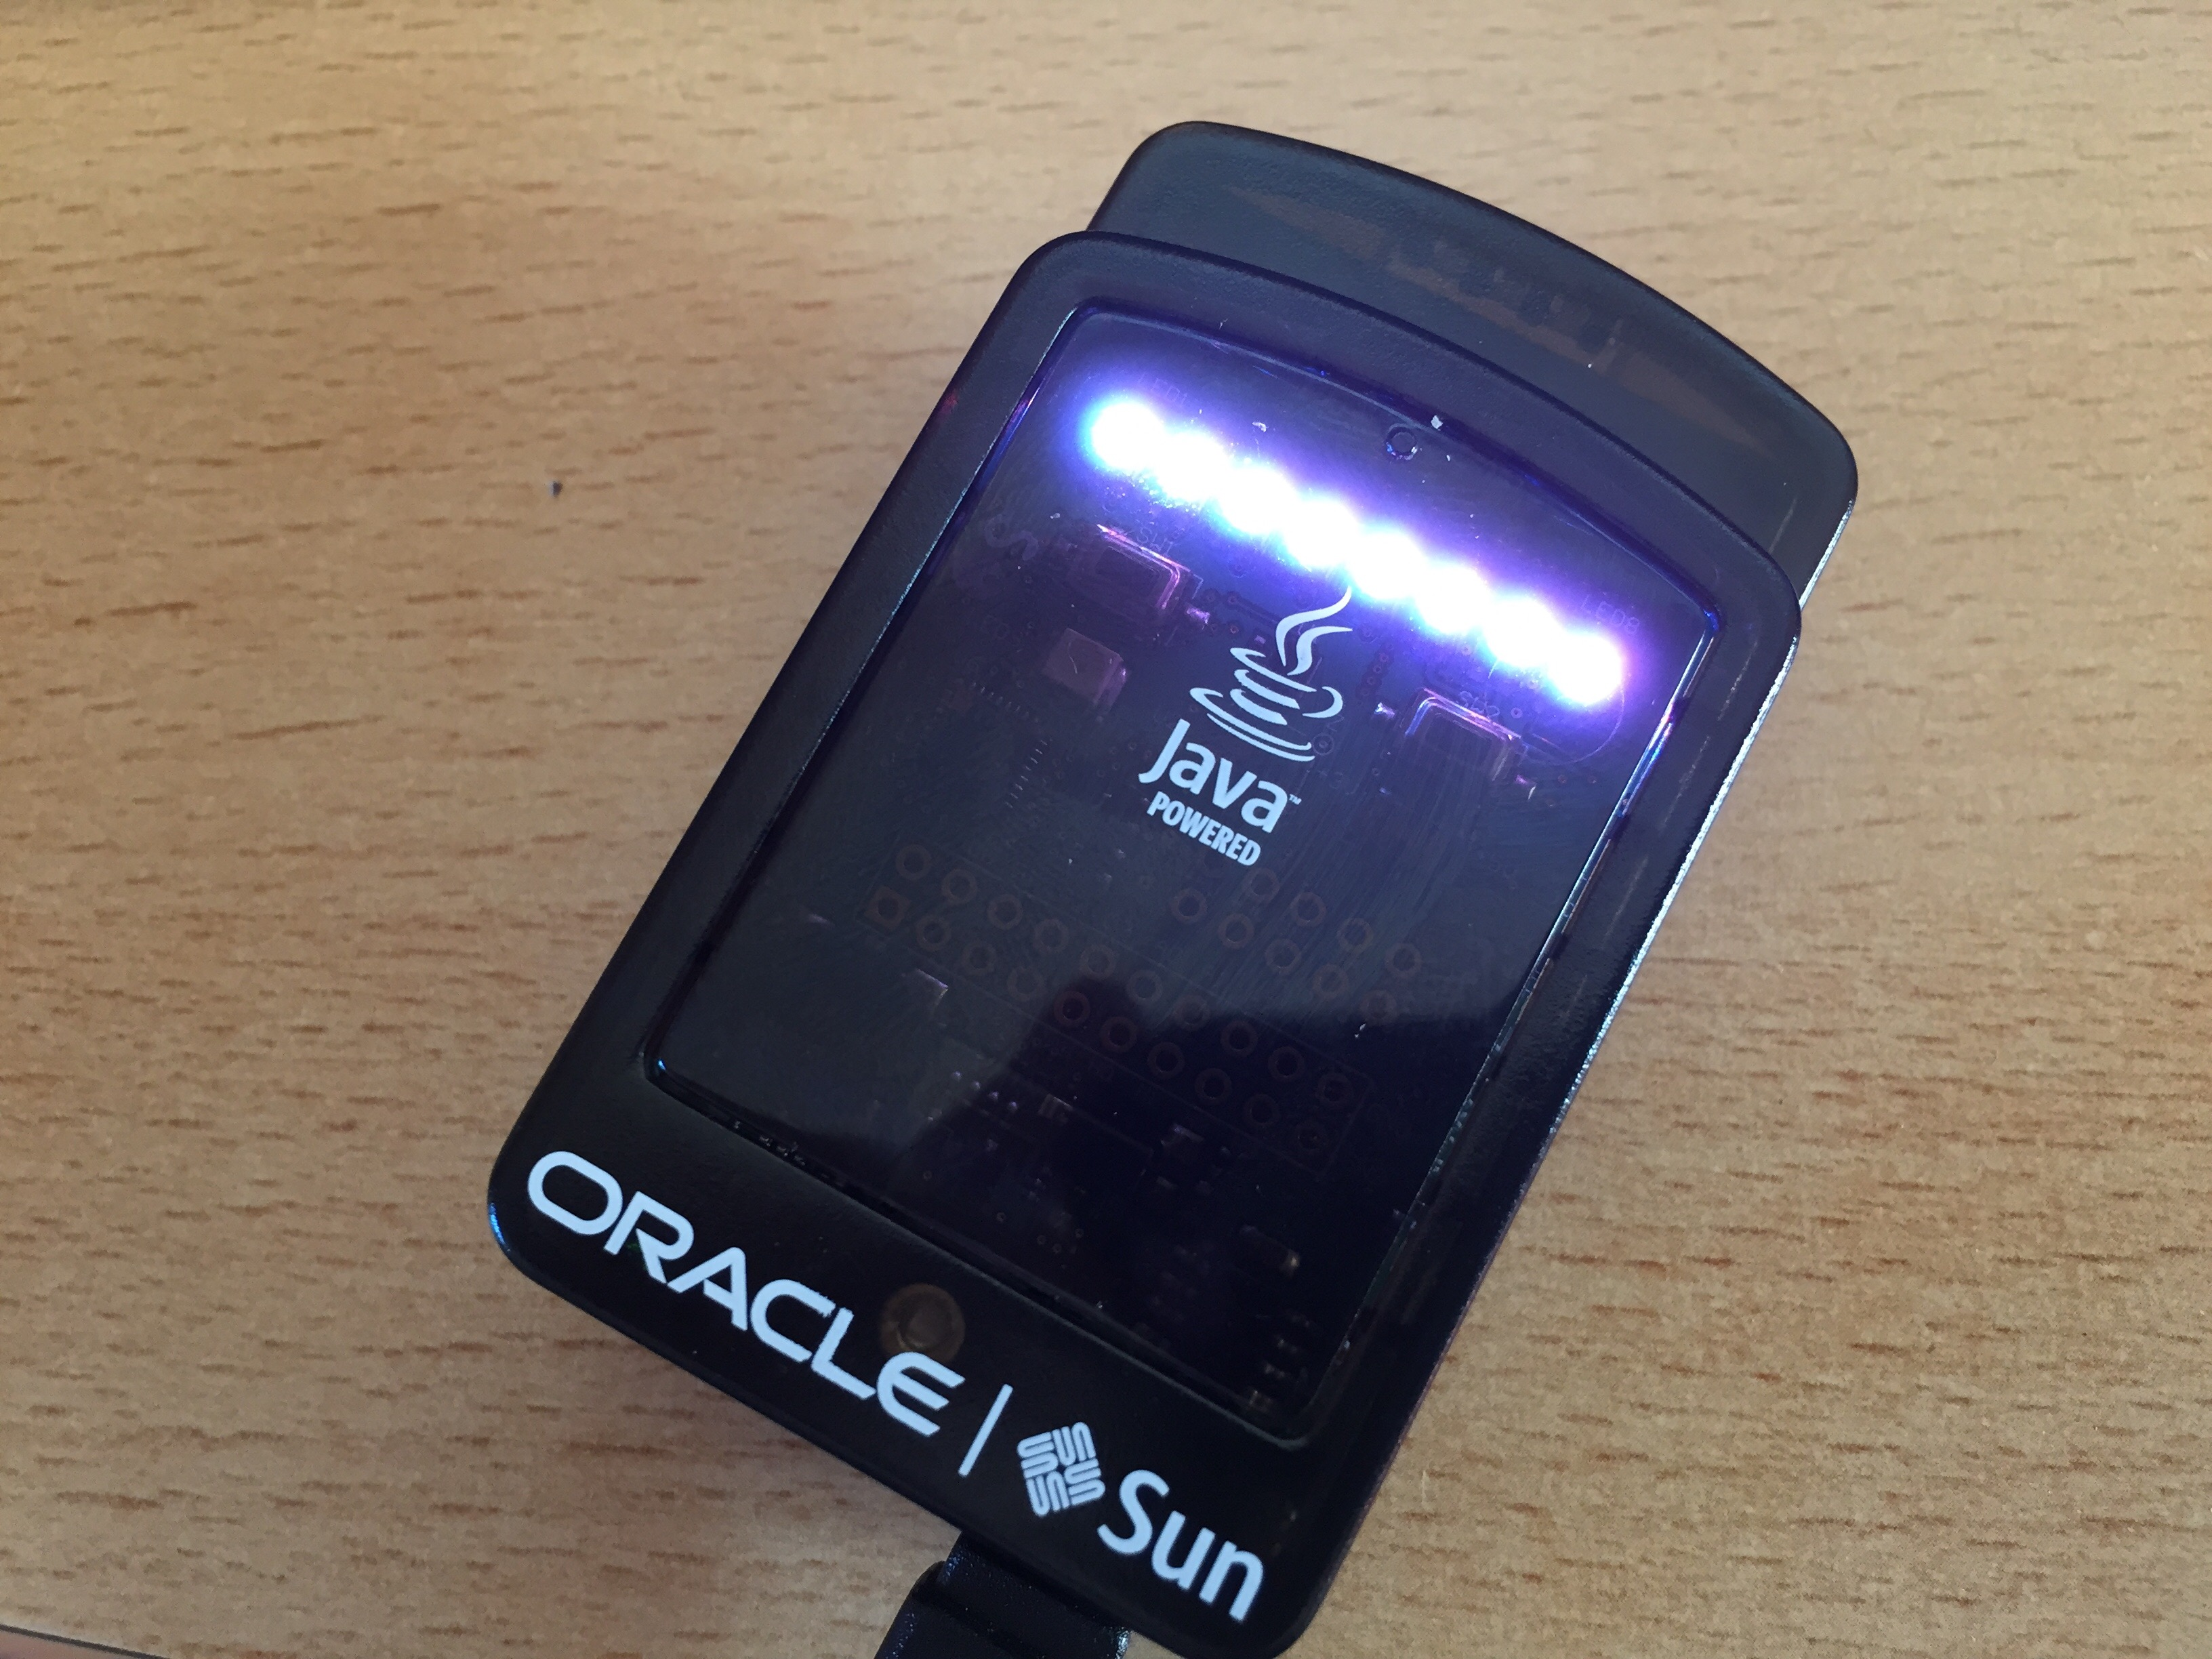
\includegraphics[scale=0.08]{Bilder/uebung1}
	\caption{Leuchtende LEDs des 'Flashlight'-Programms}
	\label{f:uebung1}
\end{figure}

Für die geplante Raumüberwachung ist diese Übung insofern hilfreich, als das hier der Umgang mit den LEDs und deren Verhalten auf äußere Einflüsse gezeigt wurde. In der späteren Implementierungsphase der Raumüberwachung sollen LEDs anzeigen, ob eine Bewegung und somit ein illegales Eindringen in den Raum stattfand.
